%===============================================================================
% LaTeX sjabloon voor de graduaatsproef Programmeren aan HOGENT
% Meer info op https://github.com/HoGentPRG/latex-hogent-report
%===============================================================================

\documentclass[dutch,dit,thesis]{hogentreport}

% TODO:
% - If necessary, replace the option `dit`' with your own department!
%   Valid entries are dbo, dbt, dgz, dit, dlo, dog, dsa, soa
% - If you write your thesis in English (remark: only possible after getting
%   explicit approval!), remove the option "dutch," or replace with "english".

\usepackage{lipsum} % For blind text, can be removed after adding actual content

%% Pictures to include in the text can be put in the graphics/ folder
\graphicspath{{../graphics/}}
%% For source code highlighting, requires pygments to be installed
%% Compile with the -shell-escape flag!
%% \usepackage[chapter]{minted}
%% If you compile with the make_thesis.{bat,sh} script, use the following
%% import instead:
\usepackage[chapter]{minted}
\usemintedstyle{solarized-light}

%% Formatting for minted environments.
\setminted{%
    autogobble,
    frame=lines,
    breaklines,
    linenos,
    tabsize=4
}

%% Ensure the list of listings is in the table of contents
\renewcommand\listoflistingscaption{%
    \IfLanguageName{dutch}{Lijst van codefragmenten}{List of listings}
}
\renewcommand\listingscaption{%
    \IfLanguageName{dutch}{Codefragment}{Listing}
}
\renewcommand*\listoflistings{%
    \cleardoublepage\phantomsection\addcontentsline{toc}{chapter}{\listoflistingscaption}%
    \listof{listing}{\listoflistingscaption}%
}

% Other packages not already included can be imported here
\usepackage{xcolor}
\usepackage{titlesec}

\definecolor{donkerrood}{RGB}{165, 42, 46}
\colorlet{title}{donkerrood}

\titleformat{\chapter}[display]{\normalfont\huge\bfseries\color{donkerrood}}{\chaptertitlename\ \thechapter}{20pt}{\Huge}
\titleformat{\section}{\normalfont\Large\bfseries\color{donkerrood}}{\thesection}{1em}{}
\titleformat{\subsection}{\normalfont\large\bfseries\color{donkerrood}}{\thesubsection}{1em}{}
\titleformat{\subsubsection}{\normalfont\normalsize\bfseries\color{donkerrood}}{\thesubsubsection}{1em}{}

\renewcommand{\contentsname}{\color{donkerrood}\IfLanguageName{dutch}{Inhoud}{Contents}}
\renewcommand{\listfigurename}{\color{donkerrood}\IfLanguageName{dutch}{Lijst van figuren}{List of figures}}
\renewcommand{\listtablename}{\color{donkerrood}\IfLanguageName{dutch}{Lijst van tabellen}{List of tables}}
\renewcommand{\listoflistingscaption}{\color{donkerrood}\IfLanguageName{dutch}{Lijst van codefragmenten}{List of listings}}

\hypersetup{colorlinks=true,linkcolor=donkerrood,citecolor=donkerrood,urlcolor=donkerrood}

%%---------- Document metadata -------------------------------------------------
% TODO: Replace this with your own information
\author{Jonas De Pus}
\supervisor{Dhr. W. Delvaux}
\cosupervisor{Dhr. K. Casier}
\title{Automatisering van Release-verificatie binnen de Amaron Releasecyclus.}
\academicyear{\advance\year by -1 \the\year--\advance\year by 1 \the\year}
\examperiod{1}
\degreesought{\IfLanguageName{dutch}{Graduaat in het Programmeren}{Associate of applied computer science}}
\partialthesis{false} %% To display 'in partial fulfilment'
%\institution{Internshipcompany BVBA.}

%% Add global exceptions to the hyphenation here
\hyphenation{back-slash}

%% The bibliography (style and settings are  found in hogentthesis.cls)
\addbibresource{gradproef.bib}            %% Bibliography file   ------------------------------------
\defbibheading{bibempty}{}

%% Prevent empty pages for right-handed chapter starts in twoside mode
\renewcommand{\cleardoublepage}{\clearpage}

\renewcommand{\arraystretch}{1.2}

%% Content starts here.
\begin{document}

%---------- Front matter -------------------------------------------------------

\frontmatter

\hypersetup{pageanchor=false} %% Disable page numbering references
%% Render a Dutch outer title page if the main language is English
\IfLanguageName{english}{%
    %% If necessary, information can be changed here
    \degreesought{Graduaat in het Programmeren}%
    \begin{otherlanguage}{dutch}%
       \maketitle%
    \end{otherlanguage}%
}{}

%% Generates title page content
\maketitle
\hypersetup{pageanchor=true}

%%=============================================================================
%% Voorwoord
%%=============================================================================

\chapter*{\IfLanguageName{dutch}{Woord vooraf}{Preface}}%
\label{ch:voorwoord}

%% TODO:
%% Het voorwoord is het enige deel van de graduaatsproef waar je vanuit je
%% eigen standpunt (``ik-vorm'') mag schrijven. Je kan hier bv. motiveren
%% waarom jij het onderwerp wil bespreken.
%% Vergeet ook niet te bedanken wie je geholpen/gesteund/... heeft

Voor u ligt de graduaatsproef "Automatisatie van het Release Verificatieproces". Dit rapport vormt het sluitstuk van mijn opleiding Graduaat Programmeren aan Hogent.

Van februari tot en met juni 2026 heb ik met veel enthousiasme stage gelopen bij het softwarebedrijf Amaron. Tijdens deze periode kreeg ik de kans om me te verdiepen in de complexe, maar fascinerende wereld van DevOps en release management. De opdracht om een geautomatiseerd verificatieplatform te ontwikkelen voor hun groeiende ecosysteem van componenten was een behowelijke technische uitdaging, maar bovenal een enorm leerzaam proces. Ik heb niet alleen mijn technische vaardigheden rondom API's en automatisering sterk kunnen verbeteren, maar ook geleerd hoe cruciaal goede communicatie en gestroomlijnde workflows zijn binnen een groot ontwikkelteam.

Dit eindwerk was echter niet tot stand gekomen zonder de hulp, begeleiding en steun van een aantal mensen die ik hier graag in de bloemetjes wil zetten.

In de eerste plaats wil ik mijn stagebegeleider bij Amaron, Koen Casier, bedanken. Bedankt voor de tijd, de technische inzichten en het vertrouwen dat ik kreeg om zelfstandig aan dit project te werken. Daarnaast wil ik ook het volledige DevOps-team en de developers van Amaron bedanken voor de warme ontvangst, de fijne samenwerking en het beantwoorden van mijn vele vragen.

Ik hoop dat u dit rapport met evenveel plezier leest als ik heb gehad bij het realiseren van dit project.
%%=============================================================================
%% Samenvatting
%%=============================================================================

% TODO: De "abstract" of samenvatting is een kernachtige (~ 1 blz. voor een
% thesis) synthese van het document.
%
% Een goede abstract biedt een kernachtig antwoord op volgende vragen:
%
% 1. Waarover gaat de graduaatsproef?
% 2. Waarom heb je er over geschreven?
% 3. Hoe heb je het onderzoek uitgevoerd?
% 4. Wat waren de resultaten? Wat blijkt uit je onderzoek?
% 5. Wat betekenen je resultaten? Wat is de relevantie voor het werkveld?
%
% Daarom bestaat een abstract uit volgende componenten:
%
% - inleiding + kaderen thema
% - probleemstelling
% - (centrale) onderzoeksvraag
% - onderzoeksdoelstelling
% - methodologie
% - resultaten (beperk tot de belangrijkste, relevant voor de onderzoeksvraag)
% - conclusies, aanbevelingen, beperkingen
%
% LET OP! Een samenvatting is GEEN voorwoord!

%%---------- Nederlandse samenvatting -----------------------------------------
%
% TODO: Als je je graduaatsproef in het Engels schrijft, moet je eerst een
% Nederlandse samenvatting invoegen. Haal daarvoor onderstaande code uit
% commentaar.
% Wie zijn/haar graduaatsproef in het Nederlands schrijft, kan dit negeren, de inhoud
% wordt niet in het document ingevoegd.



%%---------- Samenvatting -----------------------------------------------------
% De samenvatting in de hoofdtaal van het document

\chapter*{\IfLanguageName{dutch}{Samenvatting}{Abstract}}

Binnen de softwareontwikkeling bij Amaron wordt gewerkt met een vaste releasecyclus van twee tot vier weken. Het bedrijf is opgebouwd uit een ecosysteem van inmiddels circa 40 verschillende componenten en modules, die gebundeld in de hoofdrelease worden uitgerold. Voorafgaand aan elke release is momenteel een handmatige controle vereist om te bepalen of al deze onderliggende modules gereed en compleet zijn voor integratie. Dit verificatieproces zorgt voor vele frustraties en is door de groeiende omvang van het ecosysteem tijdrovend en foutgevoelig geworden. Het gebrek aan een centraal overzicht leidt tot vertragingen in de doorlooptijd van de hoofdrelease, miscommunicatie en aanzienlijke frustraties binnen het ontwikkelteam.

Om de efficiëntie en betrouwbaarheid van het releaseproces te waarborgen, is in deze graduaatsproef een geautomatiseerd verificatieplatform ontwikkeld. De realisatie hiervan is stapsgewijs en modulair aangepakt, waarbij verschillende API-koppelingen en automatiseringslogica zijn opgebouwd. Binnen de nieuwe workflow registreren developers zelf een component zodra deze gereed is. Na het doorlopen van alle automatische stappen en controles bundelt het platform deze data tot één centraal en overzichtelijk dashboard. Hierdoor kan het DevOps-team in één oogopslag effectief zien welke componenten gereed zijn en meegenomen moeten worden in de aankomende release.

Hoewel het platform zich momenteel in de eindfase van het testproces bevindt, wijzen de eerste validaties op een sterke verbetering. Het systeem slaagt erin de status van de componenten onafhankelijk te verifiëren, waardoor de menselijke foutgevoeligheid en de tijd die benodigd is voor handmatige controles drastisch worden gereduceerd. De introductie van dit platform zorgt ervoor dat de componentregistratie en het releasebeheer aanzienlijk gestroomlijnder verlopen. Door de automatisering verdwijnt de complexiteit van de handmatige checks. Dit resulteert in een kortere doorlooptijd van releases, een vlottere interne communicatie en een duidelijke afname van de frustraties op de werkvloer. Hiermee is een schaalbare oplossing gecreëerd waarmee Amaron ook in de toekomst een groeiend aantal componenten efficiënt kan blijven beheren.

%---------- Inhoud, lijst figuren, ... -----------------------------------------

\tableofcontents

% In a list of figures, the complete caption will be included. To prevent this,
% ALWAYS add a short description in the caption!
%
%  \caption[short description]{elaborate description}
%
% If you do, only the short description will be used in the list of figures

\listoffigures

% If you included tables and/or source code listings, uncomment the appropriate
% lines.
%\listoftables

%\listoflistings

% Als je een lijst van afkortingen of termen wil toevoegen, dan hoort die
% hier thuis. Gebruik bijvoorbeeld de ``glossaries'' package.
% https://www.overleaf.com/learn/latex/Glossaries

%---------- Kern ---------------------------------------------------------------

\mainmatter{}

% De eerste hoofdstukken van een graduaatsproef zijn meestal een inleiding op
% het onderwerp, literatuurstudie en verantwoording methodologie.
% Aarzel niet om een meer beschrijvende titel aan deze hoofdstukken te geven of
% om bijvoorbeeld de inleiding en/of stand van zaken over meerdere hoofdstukken
% te verspreiden!

%%=============================================================================
%% Inleiding
%%=============================================================================

\chapter{\IfLanguageName{dutch}{Inleiding}{Introduction}}%
\label{ch:inleiding}

Binnen de moderne softwareontwikkeling is een efficiënt en betrouwbaar releaseproces cruciaal om kwalitatieve oplossingen snel tot bij de eindgebruiker te krijgen. Bij het softwarebedrijf Amaron wordt gewerkt met een vaste releasecyclus van twee tot vier weken. Het bedrijf is opgebouwd uit een ecosysteem van inmiddels circa 40 verschillende componenten en modules, die gebundeld in de hoofdrelease worden uitgerold. 

Naarmate dit ecosysteem is gegroeid, is de complexiteit van het releasebeheer evenredig toegenomen. Waar in het verleden het overzicht eenvoudig te behouden was, vereist de huidige schaal een meer gestructureerde aanpak. Deze graduaatsproef richt zich op de optimalisatie en automatisering van dit specifieke onderdeel binnen de releasecyclus van Amaron.

\section{\IfLanguageName{dutch}{Probleemstelling}{Problem Statement}}%
\label{sec:probleemstelling}

Voorafgaand aan elke release is momenteel een handmatige controle vereist om te bepalen of alle onderliggende componenten gereed en compleet zijn voor integratie. Dit verificatieproces zorgt voor vele frustraties en is door de groeiende omvang van het ecosysteem tijdrovend en foutgevoelig geworden. Het gebrek aan een centraal overzicht leidt tot vertragingen in de doorlooptijd van de hoofdrelease en miscommunicatie. 

De directe doelgroep voor de oplossing van dit probleem bevindt zich intern bij Amaron. Specifiek gaat het om:

\begin{itemize}
  \item \textbf{Het DevOps-team:} Zij zijn verantwoordelijk voor de uiteindelijke uitrol en hebben momenteel geen accuraat, realtime overzicht van welke componenten klaar zijn voor de release.
  \item \textbf{De softwareontwikkelaars (developers):} Zij besteden momenteel te veel tijd aan communicatie en handmatige afstemming over de status van hun afgewerkte componenten.
\end{itemize}

\section{\IfLanguageName{dutch}{Onderzoeksvraag}{Research question}}%
\label{sec:onderzoeksvraag}

Om het bovengenoemde probleem op te lossen, is de volgende centrale onderzoeksvraag geformuleerd:

\textbf{``Hoe kan het handmatige verificatieproces voor de release van softwarecomponenten binnen Amaron efficiënt en foutloos geautomatiseerd worden?''}

Om deze centrale vraag te beantwoorden, is deze opgesplitst in de volgende deelvragen:

\begin{enumerate}
  \item Wat zijn de huidige technische en procesmatige knelpunten in de handmatige releasevoorbereiding?
  \item Welke API-koppelingen en automatiseringslogica zijn vereist om de status van een component onafhankelijk te verifiëren?
  \item Hoe kan de samenwerking tussen developers en het DevOps-team gestroomlijnd worden via een centraal dashboard?
\end{enumerate}

\section{\IfLanguageName{dutch}{Onderzoeksdoelstelling}{Research objective}}%
\label{sec:onderzoeksdoelstelling}

Het beoogde resultaat van deze graduaatsproef is de oplevering van een functionerend verificatieplatform (een werkend prototype) dat geïntegreerd is in de bestaande workflow van Amaron. 

Het project wordt als succesvol beschouwd wanneer aan de volgende criteria is voldaan:

\begin{itemize}
  \item Developers kunnen een afgewerkt component eenvoudig zelf registreren.
  \item Het DevOps-team kan in één oogopslag bepalen welke componenten meegenomen moeten worden in de release.
\end{itemize}

\section{\IfLanguageName{dutch}{Opzet van deze graduaatsproef}{Structure of this associate thesis}}%
\label{sec:opzet-graduaatsproef}

De rest van deze graduaatsproef is als volgt opgebouwd:

In Hoofdstuk~\ref{ch:stand-van-zaken} wordt een overzicht gegeven van de stand van zaken binnen het onderzoeksdomein, op basis van een literatuurstudie.

In Hoofdstuk~\ref{ch:methodologie} wordt de methodologie toegelicht en worden de gebruikte onderzoekstechnieken besproken om een antwoord te kunnen formuleren op de onderzoeksvragen.

In Hoofdstuk~\ref{ch:realisatie} wordt de technische realisatie en implementatie van het platform besproken. Hierin komen de architectuur, de opbouw van de API-koppelingen en de creatie van het dashboard aan bod. \textbf{(Let op: pas het label `ch:realisatie` aan naar het werkelijke label van jouw implementatiehoofdstuk, indien dit anders heet).}

In Hoofdstuk~\ref{ch:conclusie}, tenslotte, wordt de conclusie gegeven en een antwoord geformuleerd op de onderzoeksvragen. Daarbij wordt ook een aanzet gegeven voor toekomstig onderzoek binnen dit domein.
\chapter{\IfLanguageName{dutch}{Stand van zaken}{State of the art}}%
\label{ch:stand-van-zaken}

In het vorige hoofdstuk werd de probleemstelling rondom het handmatige en foutgevoelige releaseproces bij Amaron toegelicht. Om een gerichte en toekomstbestendige oplossing te kunnen ontwerpen, is een goed begrip van de onderliggende technologieën, best practices en methodieken essentieel. Dit hoofdstuk schetst de theoretische achtergrond en de huidige stand van zaken binnen de domeinen van release management, automatisering en API-integraties. Deze literatuurstudie vormt de fundering voor de keuzes die in Hoofdstuk~\ref{ch:methodologie} (Methodologie) en de uiteindelijke realisatie worden gemaakt.

\begin{figure}
  \centering
  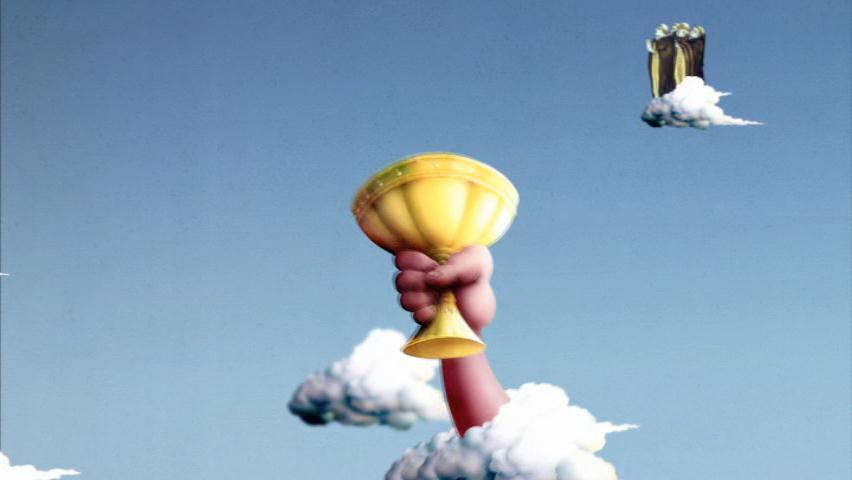
\includegraphics[width=0.8\textwidth]{grail.jpg}
  \caption[Voorbeeld figuur.]{\label{fig:grail}Voorbeeld van invoegen van een figuur. Zorg altijd voor een uitgebreid bijschrift dat de figuur volledig beschrijft zonder in de tekst te moeten gaan zoeken. Vergeet ook je bronvermelding niet!}
\end{figure}

\begin{listing}[htbp]
\begin{minted}[autogobble,breaklines,linenos,frame=lines,tabsize=4]{python}
import pandas as pd
import seaborn as sns

penguins = sns.load_dataset('penguins')
sns.relplot(data=penguins, x="flipper_length_mm", y="bill_length_mm", hue="species")
\end{minted}
  \caption[Voorbeeld codefragment]{\label{lst:penguins}Voorbeeld van het invoegen van een codefragment.}
\end{listing}

\lipsum[7-20]

\begin{table}
  \centering
  \begin{tabular}{lcr}
    \toprule
    \textbf{Kolom 1} & \textbf{Kolom 2} & \textbf{Kolom 3} \\
    $\alpha$         & $\beta$          & $\gamma$         \\
    \midrule
    A                & 10.230           & a                \\
    B                & 45.678           & b                \\
    C                & 99.987           & c                \\
    \bottomrule
  \end{tabular}
  \caption[Voorbeeld tabel]{\label{tab:example}Voorbeeld van een tabel.}
\end{table}


%%=============================================================================
%% Methodologie
%%=============================================================================

\chapter{\IfLanguageName{dutch}{Methodologie}{Methodology}}%
\label{ch:methodologie}

Om de onderzoeksvraag te beantwoorden en het handmatige verificatieproces succesvol te automatiseren, is gekozen voor een stapsgewijze en iteratieve aanpak. Door het project op te delen in overzichtelijke fasen, kon de overgang van de initiele data-analyse naar de uiteindelijke integratie in de gebruikersflow gestructureerd verlopen. Dit hoofdstuk geeft een beknopt overzicht van deze fasen, de bijbehorende doelstellingen en de opgeleverde resultaten (deliverables). 

De werkelijke technische realisatie en de details van deze stappen worden verder uitgediept in het volgende hoofdstuk.

\section{\IfLanguageName{dutch}{Behoefteanalyse en Datamodellering}{Phase 1: Requirements Analysis and Data Modeling}}%
\label{sec:methode-fase1}

De eerste fase van het project richtte zich op het in kaart brengen van de benodigde informatie. Om een component succesvol te kunnen registreren voor een release, moest eerst exact bepaald worden welke data het systeem nodig had. 

\begin{itemize}
  \item \textbf{Doelstelling:} Het bepalen van de benodigde invoerdata en het ontwerpen van een formulier waarmee developers deze data efficiënt kunnen aanleveren.
  \item \textbf{Methode:} Een analyse van het bestaande handmatige proces om te bepalen welke variabelen cruciaal zijn voor de rest van de workflow.
  \item \textbf{Deliverable:} Een gedefinieerd datamodel en de velden voor een registratieformulier dat als startpunt van de automatisering dient.
\end{itemize}

\section{\IfLanguageName{dutch}{API-analyse en Backend-ontwikkeling}{Phase 2: API Analysis and Backend Development}}%
\label{sec:methode-fase2}

Zodra duidelijk was welke data via het formulier werd verzameld, moest worden vastgesteld hoe deze data verwerkt diende te worden. Dit vereiste interactie met verschillende achterliggende systemen via API's. 

\begin{itemize}
  \item \textbf{Doelstelling:} Het faciliteren van de juiste acties op basis van de ingevoerde formulierdata.
  \item \textbf{Methode:} Het uitvoeren van een gap-analyse tussen de reeds bestaande API's binnen Amaron en de API's die nog ontbraken voor dit specifieke verificatieproces. Waar functionaliteit ontbrak, werden nieuwe, specifieke API-endpoints geschreven en getest.
  \item \textbf{Deliverable:} Een set van werkende API-koppelingen die de data kunnen wegschrijven, ophalen en valideren.
\end{itemize}

\section{\IfLanguageName{dutch}{Integratie en Workflow-optimalisatie}{Phase 3: Integration and Workflow Optimization}}%
\label{sec:methode-fase3}

Met de backend-logica (API's) en de frontend-invoer (het formulier) op hun plek, was de volgende logische stap het samenvoegen van deze elementen tot één vloeiend proces. Hierbij was de gebruikerservaring (UX) voor de developers van groot belang.

\begin{itemize}
  \item \textbf{Doelstelling:} Het naadloos integreren van de ontwikkelde API's in de algehele flow, zodat het proces voor de eindgebruiker zo vlot en intuïtief mogelijk verloopt.
  \item \textbf{Methode:} Nauwe samenwerking en afstemming met de interaction designer. De technische API-calls werden gekoppeld aan de visuele flow-stappen die door de designer waren uitgetekend.
  \item \textbf{Deliverable:} Een geautomatiseerde, werkende workflow waarin dataregistratie en achtergrondverwerking succesvol geïntegreerd zijn.
\end{itemize}

\begin{center}
  \captionsetup{type=figure}
  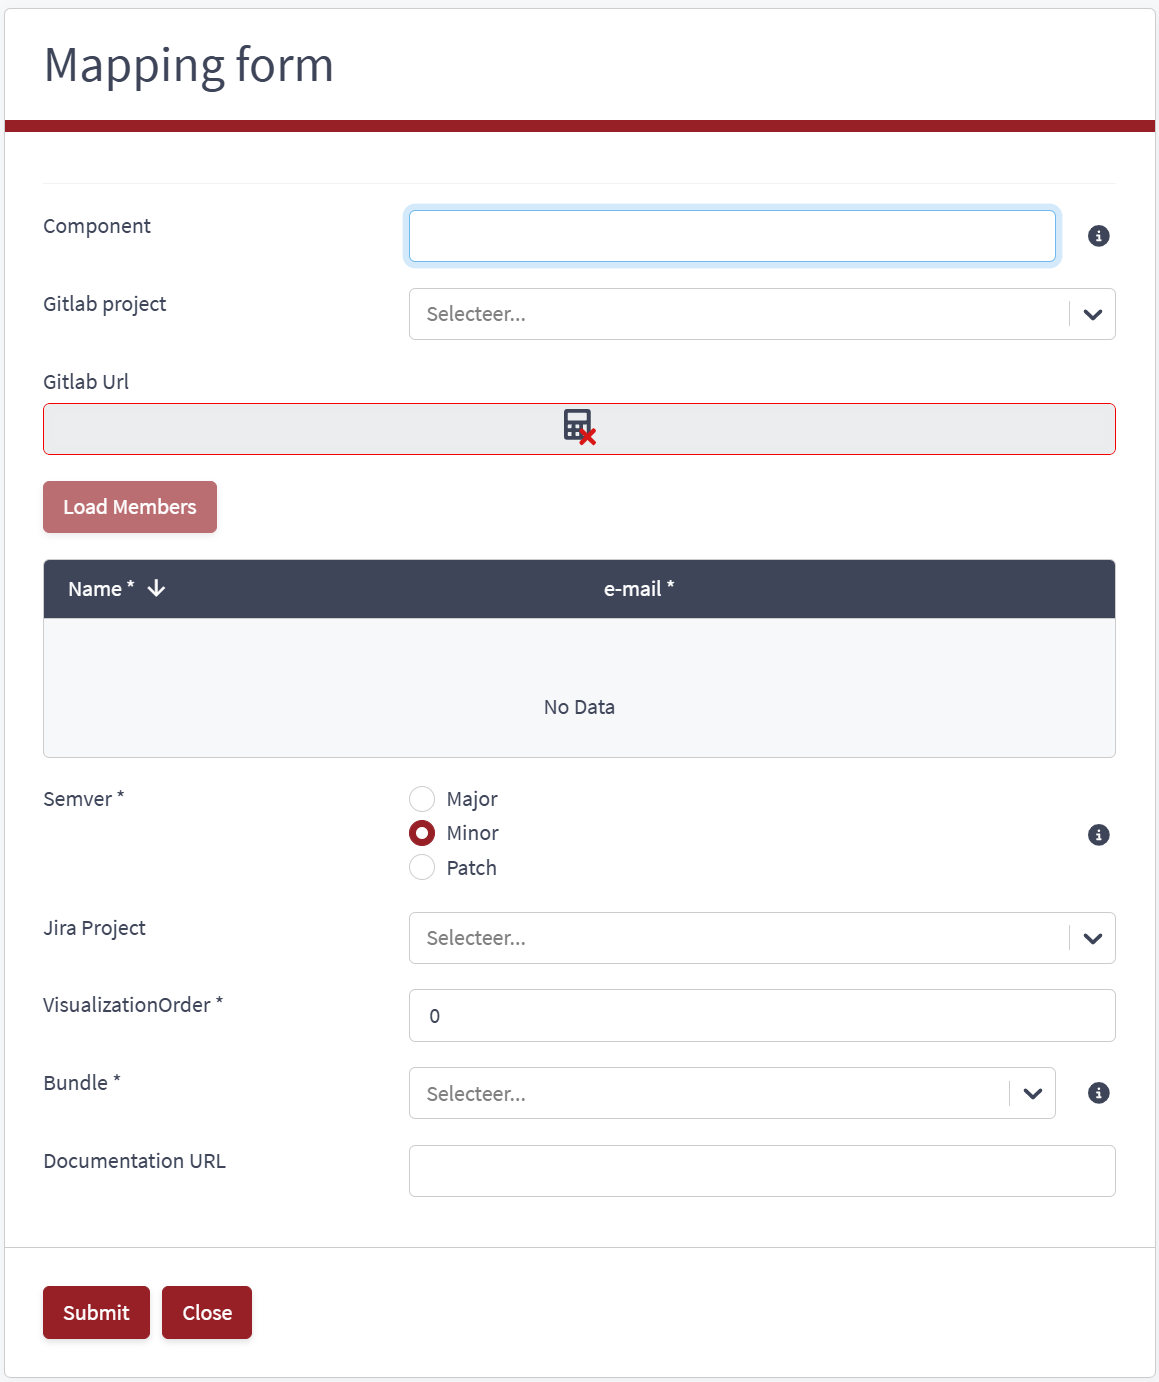
\includegraphics[width=0.9\linewidth]{form}
  \captionof{figure}[Formulierinterface]{Dit voorbeeld toont de interface van een formulier, voorzien van diverse gegevensvelden voor zowel datavisualisatie als gebruikersinvoer, aangevuld met actieknoppen voor navigatie en functie-uitvoering.}
\end{center}

\begin{center}
  \captionsetup{type=figure}
  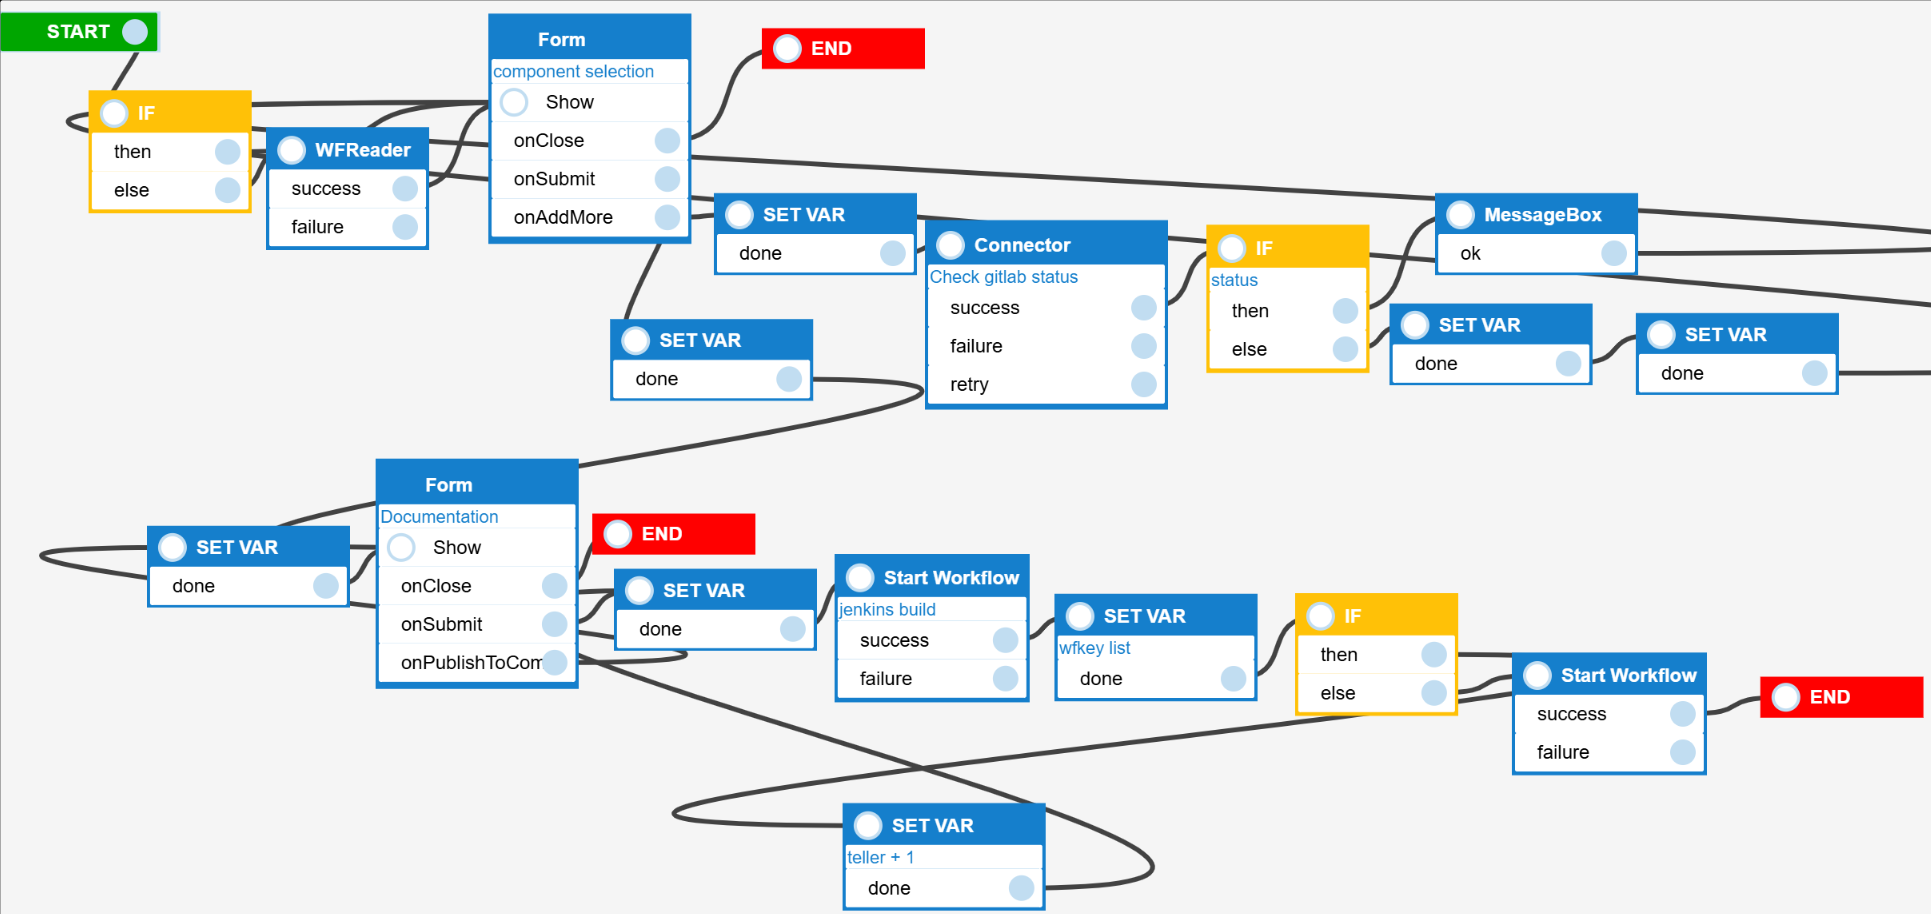
\includegraphics[width=1.0\linewidth]{id}
  \captionof{figure}[Interaction designer]{Op de bijgevoegde screenshot zie je de visuele weergave van de interaction designer. Deze opzet illustreert mooi hoe de verschillende elementen met elkaar verbonden zijn om complexe handelingen op de achtergrond te stroomlijnen.}
\end{center}

\section{\IfLanguageName{dutch}{Testen en Validatie}{Phase 4: Testing and Validation}}%
\label{sec:methode-fase4}

In de afrondende fase wordt de gebouwde proof of concept (PoC) gevalideerd in de praktijk.

\begin{itemize}
  \item \textbf{Doelstelling:} Controleren of de ontwikkelde workflow daadwerkelijk de frustraties en tijdsverspilling van het handmatige proces oplost.
  \item \textbf{Methode:} Functioneel testen van de componentenregistratie en het genereren van het uiteindelijke release-overzicht voor het DevOps-team.
  \item \textbf{Deliverable:} Een gevalideerd verificatieplatform klaar voor verdere uitrol of iteratie.
\end{itemize}

% Voeg hier je eigen hoofdstukken toe die de ``corpus'' van je graduaatsproef
% vormen. De structuur en titels hangen af van je eigen onderzoek. Je kan bv.
% elke fase in je onderzoek in een apart hoofdstuk bespreken.

%\input{...}
%\input{...}
%...

%%=============================================================================
%% Conclusie
%%=============================================================================

\chapter{Conclusie}%
\label{ch:conclusie}

Deze graduaatsproef is gestart vanuit een concrete en urgente behoefte binnen Amaron: het stroomlijnen van een releaseproces dat, door de groei naar een ecosysteem van circa 40 componenten, te complex, tijdrovend en frustrerend was geworden. Het handmatig verifiëren van de status van elk component zorgde voor een bottleneck bij het DevOps-team en onnodige communicatie-overhead voor de developers. 

\section{Beantwoording van de onderzoeksvraag}

De centrale onderzoeksvraag van dit project luidde: \textit{``Hoe kan het handmatige verificatieproces voor de release van softwarecomponenten binnen Amaron efficiënt en foutloos geautomatiseerd worden?''}

Uit de realisatie en de testfase is gebleken dat dit succesvol kan worden geautomatiseerd door een decentrale benadering te combineren met gecentraliseerde zichtbaarheid. Het antwoord op de onderzoeksvraag ligt in de ontwikkelde workflow:
\begin{itemize}
  \item \textbf{Decentrale registratie:} Developers nemen zelf de verantwoordelijkheid om een afgewerkt component te registreren via een intuïtief formulier, wat direct gekoppeld is aan de visuele flow van de interaction designer.
  \item \textbf{Geautomatiseerde verificatie:} Door het ontwikkelen en aanroepen van specifieke API's worden de noodzakelijke controles op de achtergrond uitgevoerd zonder menselijke tussenkomst.
  \item \textbf{Gecentraliseerd overzicht:} Alle gevalideerde data stroomt samen in één overzichtelijk dashboard, waardoor het DevOps-team in één oogopslag de gereedheid van de release kan beoordelen.
\end{itemize}

\section{Meerwaarde en impact}

De implementatie van dit platform biedt een aanzienlijke meerwaarde voor de interne werking van Amaron. De frustraties die gepaard gingen met het constant moeten navragen van statussen zijn weggenomen. Voor de developers betekent dit minder onderbrekingen in hun werk, en voor het DevOps-team betekent het een drastische reductie in voorbereidingstijd voor een release. Bovendien is de foutgevoeligheid geminimaliseerd, omdat de controle nu leunt op objectieve data uit API's in plaats van op menselijke interpretatie of handmatige checklists.

\section{Kritische reflectie}

Hoewel het ontwikkelde systeem de vooropgestelde doelen behaalt, is een kritische blik op het resultaat op zijn plaats. De automatisering werkt technisch naar behoren, maar het succes van het platform is sterk afhankelijk van de adoptie door de gebruikers. Als developers vergeten het registratieformulier in te vullen, is het overzicht voor DevOps alsnog incompleet. De oplossing is momenteel dus nog deels afhankelijk van een menselijke handeling aan de start van de flow. Daarnaast bevond het platform zich aan het einde van dit onderzoek nog in de afrondende testfase, waardoor langetermijndata over de daadwerkelijke tijdwinst per releasecyclus nog verder gekwantificeerd moet worden.

\section{Aanbevelingen en toekomstig onderzoek}

Dit project heeft een solide basis gelegd voor geautomatiseerd releasebeheer binnen Amaron, maar opent ook deuren voor verdere optimalisatie. Voor de toekomst worden de volgende stappen aanbevolen:
\begin{itemize}
  \item \textbf{Volledige CI/CD integratie:} Onderzoeken of de initiële registratiestap door de developer volledig weggenomen kan worden, door deze trigger in te bouwen in de bestaande CI/CD pipelines (bijvoorbeeld automatisch registreren bij een specifieke Git-merge).
  \item \textbf{Uitbreiding van API-controles:} Het toevoegen van meer diepgaande kwaliteitscontroles, zoals het automatisch ophalen van security scans of test coverage rapporten voordat een component als `gereed` wordt gemarkeerd op het dashboard.
  \item \textbf{Gefaseerde uitrol:} Het systeem stapsgewijs uitrollen voor alle 40+ componenten, begeleid door duidelijke documentatie en training voor de developers om de adoptie te garanderen.
\end{itemize}

Samenvattend is met dit project een belangrijke stap gezet in de professionalisering en schaalbaarheid van het releaseproces bij Amaron, waarmee een solide technische basis is gelegd voor toekomstige groei.

%---------- Backmatter, referentielijst ---------------------------------------

\backmatter{}

\setlength\bibitemsep{2pt} %% Add Some space between the bibliograpy entries
\nocite{Humble2010,Fowler2006,Newman2015}
\printbibliography[heading=bibintoc]

\end{document}
